

\paragraph{} In this chapter we shall introduce and detail a prototype implementation of a modular, \acrshort{sgx}-protected \textit{reference monitor} --- \textsc{Citadel}. We start by considering this project's motivation and discussing the challenges faced. Then, we explain the three-part architecture, relating design decisions to its \acrshort{difc} model. We discuss the architecture's performance and effectiveness in §~\ref{sec:eval}.

\section{Motivation}
\paragraph{} Since its introduction in Anderson's 1972 report,~\cite{reference-monitor} the reference monitor concept has proved a reliable workhorse for many security models. It does not refer to any exact policy, nor limit itself to any particular implementation --- its abstractness is one of its greatest strengths, reserving any judgement about what policy is \textit{appropriate} in a particular setting.~\cite{irvine-rm}

\paragraph{Fundamental Properties of a Reference Monitor}

\begin{itemize}
    \item \textit{Always invoked.} To guarantee that adversaries are unable to bypass the system's security policies, every access to the system must be mediated
    \item \textit{Evaluable.} It ``must be small enough to be subject to analysis and tests, the completeness of which can be assured'';~\cite{reference-monitor} to be trustworthy, it must be \textit{auditable}, with, ideally, a restricted \acrshort{tcb}.
    \item \textit{Tamper proof.} The integrity of a reference monitor, which presides over the system's authorisation mechanisms, cannot be in question.
\end{itemize}

\paragraph{} No computer system is ever completely secure, and Linux is no exception. Having grown by 1.7 million lines of code (\acrshort{loc}) in the past year alone, to 27.8 million \acrshort{loc} in total,\footnote{\url{https://www.theregister.com/2020/01/06/linux\_2020\_kernel\_systemd\_code/}} bugs are inevitable --- almost 2000 have been reported in the past year,\footnote{\url{https://bugzilla.kernel.org/}} and 662 \textit{severe} bugs are still outstanding.\footnote{\url{https://www.cvedetails.com/product/47/Linux-Linux-Kernel.html}} Therefore we must question whether Linux alone can provide a reference monitor implementation the guarantees it requires,~\cite{Lipp2018MeltdownRK, 10.5555/2831143.2831164} thus motivating the use of \acrshort{sgx}.

\paragraph{} Applying \acrshort{sgx} to this problem brings two attractive benefits;
\begin{itemize}
    \item The system's \acrshort{ifc} policy can be evaluated both during offline analysis and online using \textit{attestation}, building other enclaves' confidence in the underlying system.
    \item \acrshort{sgx}'s hardware protections are very capable of defending a reference monitor's state, even if adversaries have ring-0 privileges or in the presence of a kernel bug.
\end{itemize}


\section{Challenges}
\label{sec:challenges}

\begin{figure}[]
    \centering
    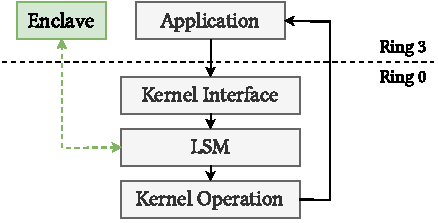
\includegraphics[width=0.48\linewidth]{figures/SGX-EnclaveIntegration.pdf}
    \caption[Abstract \textit{syscall} control flow route for enclave integration.]{Abstract \textit{syscall} control flow route. Grey components show the natural Linux design. Green additions highlight the externalised enclave LSM component.}
    \vspace{5mm}
    \label{fig:sgx-abstract-integration}
\end{figure}

\paragraph{} The natural location for a reference monitor is embedded directly into the kernel, in the path of \textit{syscalls'} control flows. \textit{CamFlow} does this using the \acrshort{lsm} framework, silently tagging processes and other entities as they are encountered by the kernel, and additionally providing an external \acrshort{lsm}-interface for any active changes. However, an \acrshort{sgx} enclave is incompatible with this workflow (§~\ref{sec:sgx-no-kernel-mode}) as it cannot execute alongside kernel code. Thus a significant, unavoidable design feature is that the reference monitor must be distributed across rings 0 and 3 --- an enclave \textit{policy} component, and an \acrshort{lsm} for \textit{enforcement}.

\paragraph{} The disruption this change causes could severely impact performance; Figure~\ref{fig:sgx-abstract-integration} highlights the significant change to overall control flow. Most notably, externalising part of the \acrshort{lsm} to an enclave forces, in the worst case, an additional pair of context switches for each \textit{syscall}.

\paragraph{} Given a ring-3 component is unavoidable, we seek to minimise the overhead caused by its integration, while maintaining \textit{safety} (every operation must be mediated). This situation is reminiscent of \textit{exokernels};~\cite{10.1145/224056.224076} forcing a portion of the system into userspace could, if treated carefully, help overall performance.~\cite{10.1145/269005.266644} 

\paragraph{} Two architectures, as illustrated in Figure~\ref{fig:sgx-integration}, were initially considered. 

\begin{enumerate}
    \item An \textit{isolated} extension of the \acrshort{lsm}. Only the security implementation communicates with the \textit{policy} enclave, acting as a na\"{i}ve reimplementation of a fully self-contained \acrshort{lsm}, and using an additional kernel module as an \acrshort{io} relay.
    \item An \textit{integrated} userspace service, through which permission is \textit{requested} ahead of time and decisions stored in the \acrshort{lsm} until needed. Backflow of information is facilitated asynchronously, but no additional kernel relay is required.
\end{enumerate}



\begin{figure}[]
    \centering
    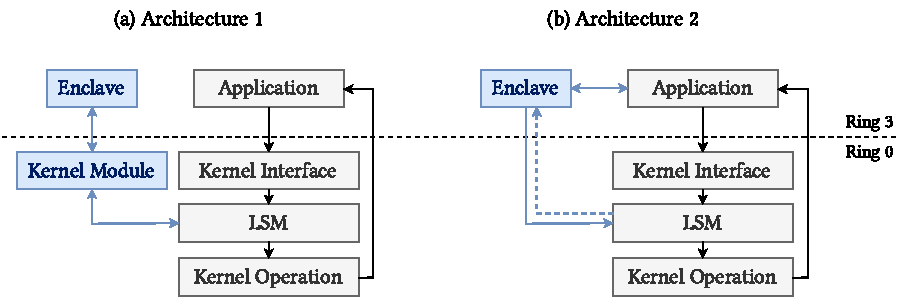
\includegraphics[width=0.98\linewidth]{figures/SGX-EnclaveIntegration-Design}
    \caption{Two possible enclave integration designs.}
    \vspace{2mm}
    \label{fig:sgx-integration}
    \vspace{5mm}
\end{figure}

\paragraph{}\textit{Architecture 1} can be implemented without changing the \acrshort{ifc} model presented in §~\ref{sec:ifc-modelling}, reducing concerns regarding correctness and safety. However it adds significant overhead to the critical sections~\cite{Dubois1988SynchronizationCA} of core \acrshort{lsm} functions, in most cases while the kernel holds locks for various objects being accessed.

\paragraph{} \textit{Architecture 2} is more flexible, requiring all negotiation be conducted ahead of time, and importantly, without leaving userspace: any overhead only impacts the application, leaving the kernel's critical sections to execute with minimal interference. A notable downside, however, is that the system's security model will need an extension because \textit{policy decisions and enforcement are no longer one and the same}.

\paragraph{} Preliminary experiments showed that performance of the two architectures was similar in light workloads, but that \textit{Architecture 1} degrades significantly due to resource contention. Additionally, as will be explained in §~\ref{sec:citadel-tcb}, the dependence on a kernel module conflicts with the desired constrained \acrshort{tcb} of the system. For these reasons \textit{Architecture 2} forms the basis of the prototype.

\paragraph{} An additional challenge is one of incomplete information --- an enclave is not privy to internal kernel datastructures such as \texttt{task\_struct}, which will store the taint and capabilities of processes. A potential solution would be a request-response model via a custom kernel interface for any queries, though the performance impact would be severe, requiring additional context switches. Instead, the approach adopted creates an abstract interface that purposefully removes the minutiae of the underlying system. Any solution must be trustworthy and safe, and malicious entities must not be able to exploit any \textit{eventually consistent} components.~\cite{10.1145/1435417.1435432}

\paragraph{} As a final comment, it must be noted that \acrshort{sgx} is not flawless; §~\ref{sec:sgx-vulnerabilities} discusses the impact of this on the project.


% ---------------
\clearpage
\section{The \textsc{Citadel} IFC Model}

\paragraph{} Before work on the final \textsc{Citadel} implementation began, we constructed a formalisation describing the distributed nature of its design. A model helps reason about the safety and correctness of the final system, and provides the notation to properly discuss its features. Our model directly extends the one presented in §~\ref{sec:ifc-modelling}.

\subsection{Reservations}

\paragraph{} Previously we defined the concept of a \textit{safe flow}, $A \rightarrow B$, which underpins our \acrshort{ifc} restrictions. In previous works permission is granted while \textit{implicitly} considering \textit{how} the flow is to take place (\ref{eqn:res-1}). An isolated \textit{enforcement} component does not understand the concept of \textit{flows}, forcing policy decisions to be defined \textit{explicitly}; \textsc{Citadel} uses \textit{reservations} for this purpose (\ref{eqn:res-2}). This distinction is simple but very important when introducing \textit{laziness} and other optimisations between the two halves of the reference monitor.

\begin{equation}\label{eqn:res-1}
    \textit{operation} \rightarrow \boxed{\textit{reference monitor}} \xrightarrow{\;\;\textit{decision}\;\;} \{0,1\}
\end{equation}
\vspace{-3mm}
\begin{equation}\label{eqn:res-2}
    \textit{operation} \rightarrow \boxed{\textit{policy}\; \xrightarrow{\;\;\textit{reservation}\;\;} \;\textit{enforcement}} \xrightarrow{\;\;\textit{decision}\;\;} \{0,1\}
    \vspace{3mm}
\end{equation}


\paragraph{} Let $\Omega$ be the set of all operations mediated by the reference monitor, for example, \texttt{file\_read} or \texttt{socket\_open}, and $\mathcal{R}$, the set of all \textit{reservations}, as follows.\footnote{Recalling that $\mathcal{T}$ is the set of all tags.}

\newcommand{\powerset}{\raisebox{.15\baselineskip}{\Large\ensuremath{\wp}}}
\vspace{-5mm}
\begin{equation*}
    \mathcal{R} = \mathcal{T} \times \powerset(\Omega)
    \vspace{2mm}
\end{equation*}

\paragraph{} Further, we define a shorthand, $t^{\alpha}$;
\vspace{-3mm}
\begin{equation*}
    r \in \mathcal{R} \;.\; (r = (t, \alpha) = t^{\alpha} \implies t \in \mathcal{T} \; \wedge \; \alpha \subseteq \Omega)
\end{equation*}

\paragraph{} For a process $A$, $A_{r} \subseteq \mathcal{R}$ defines the set of all reservations it holds. Once a decision has been made, it is important for a reference monitor to be able to change it, revoking access if required. Thus we specify \textit{validity} with an indicator function, $\mathcal{V}: \mathcal{R} \mapsto \{0,1\}$. A reservation can only be used if valid; invalid reservations are discarded.

\subsection{Permissible Operations}
\label{sec:permissible-operations}

\paragraph{Satisfiability} To determine if an operation is permissible, the \textit{constraint reservation} representing it is compared against reservations held by the process. For example, $t^{\{\texttt{file\_read}\}}$ is the constraint for reading a file tagged $t$.

\paragraph{} A constraint $\tau^{x}$ is said to be satisfied by a reservation $\tau^{y}$ ($\tau^{x} \sprecsim \tau^{y}$) if the tags match, the reservation is valid, and $y$ permits \textit{at least} the required form of access (\ref{eqn:satis-1}). 

% Equations (\ref{eqn:satis-2}) and (\ref{eqn:satis-3}) define set comparison counterparts --- constraint $\tau^{x}$ is satisfied by a set of reservations $y$ ($\tau^{x} \sqin y$), and a set of constraints $\mu$ is satisfied by a set of reservations $\nu$ ($\mu \sqsubseteq \nu$).

\vspace{-5mm}
\begin{align}
    \sigma^{\alpha}, \tau^{\beta} \in \mathcal{R} &\;.\; (\; \sigma^{\alpha} \sprecsim \tau^{\beta} \iff \sigma = \tau \;\wedge\; \alpha \subseteq \beta \;\wedge\; \mathcal{V}(\tau^{\beta}) \;) \label{eqn:satis-1}
\end{align}

% \\
% \sigma^{\alpha} \in \mathcal{R}, \; x \subseteq \mathcal{R} &\;.\;  (\; \sigma^{\alpha} \sqin x \iff \exists \, \tau^{\beta} \in x \;.\; \sigma^{\alpha} \sprecsim \tau^{\beta} \;) \label{eqn:satis-2}\\
% \mu, \nu \subseteq \mathcal{R} &\;.\;  (\; \mu \sqsubseteq \nu \iff \forall \, \alpha \in \mu \;.\; \alpha \sqin \nu \;) \label{eqn:satis-3}

\paragraph{} From here we define a \textit{permissible operation}, $A \xrightharpoonup{\;\omega\;} t$; process $A$ may perform operations $\omega$ on an entity tagged $t$. An operation is only permissible if the process holds a reservation explicitly granting permission (\ref{eqn:permissible-op}).
\begin{equation}
    \label{eqn:permissible-op}
    A \xrightharpoonup{\;\omega\;} t \iff (\exists \; t^{\alpha} \in A_r \implies t^{\omega} \sprecsim t^{\alpha})
\end{equation}

\paragraph{} To bridge the gap between permissible flows and operations, a final definition is required; a \textit{specific permissible flow}, $A \,\xmapsto{\;\omega,\tau\;}\, B$, meaning that $A$ may send information to $B$ using operations $\omega$, via entities tagged with $\tau$. Thus:

\vspace{-7mm}
\begin{align}
    (\exists\, \omega,\tau \;.\; A \,\xmapsto{\;\omega,\tau\;}\, B) \implies & A \rightarrow B \\
    A \,\xmapsto{\;\omega,\tau\;}\, B \implies & (\exists \,\omega' \;.\; A \xrightharpoonup{\;\omega'\;} \tau \;\land\; \omega \subseteq \omega') \label{eqn:flow-abs-conc-map}
\end{align}

\paragraph{} Together, these define the relationship between an abstract policy space ($A \rightarrow B$, §~\ref{sec:policy-enclave}) and concrete implementation ($A \xrightharpoonup{\;\omega\;} \tau$, §~\ref{sec:enforcement-domain}). A policy decision may grant a greater set of permissions than asked for (\ref{eqn:flow-abs-conc-map}) --- e.g. allowing both read and write when only write was explicitly requested.~\cite{flume,Zeldovich2008}

\paragraph{} Some small updates are required to make the existing rules consistent with the new: reservations are not transferred when creating a new entity (\ref{eqn:new-creation}), and reservations are not affected by capabilities as they represent a centralised component of the \acrshort{difc} system. 

\vspace{-5mm}
\begin{equation}
    A \Rightarrow B \implies A_s = B_s \; \wedge \; A_i = B_i \; \wedge \; B_r = \varnothing \label{eqn:new-creation}
\end{equation}


\subsection{Transient Entities}
\label{sec:transient-entities}

\paragraph{} Alongside active and passive entities, we introduce a third type; \textit{transient} entities. These are passive entities that are privately held by an owning active entity; they are used to model Linux functions such as \texttt{pipe()} and unclaimed tainted files.

\paragraph{} To facilitate this, all processes are assigned a unique tag $p \in \mathcal{T}$, and any files it creates are initially also be tagged with $p$. Using $\mathcal{P}$ as the set of all process identifiers, we define $\mathcal{I}$ as the function returning a process's transient identifier;

\vspace{-5mm}
\begin{equation}
    \mathcal{I}: \mathcal{P} \mapsto \mathcal{T}
\end{equation}

\paragraph{} The expression for a \textit{permissible operation} now becomes;

\vspace{-5mm}
\begin{equation}
    A \xrightharpoonup{\;\omega\;} t \iff \mathcal{I}(A) = t \;\lor\; (\exists \; t^{\alpha} \in A_r \implies t^{\omega} \sprecsim t^{\alpha})
\end{equation}

% ---------------
\clearpage
\section{Implementation}

\begin{figure}[]
    \centering
    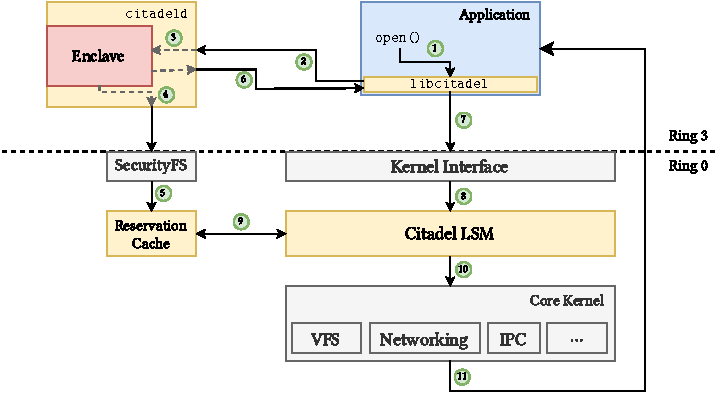
\includegraphics[width=\linewidth]{figures/OverallArchitecture.pdf}
    \caption{High level overview of the \textsc{Citadel} architecture.}
    \vspace{-5mm}
    \label{fig:citadel-overview}
    \vspace{5mm}
\end{figure}

\paragraph{} \textsc{Citadel} consists of its \acrshort{lsm}, \texttt{citadeld}, and \texttt{libcitadel}. Each plays an essential, symbiotic role in the reference monitor's operation. The prototype is over 9,000 lines of C and C++, extending the Linux kernel build system (§~\ref{sec:build-system}). This section presents \textsc{Citadel}'s architecture, guided by Figure~\ref{fig:citadel-overview}.

\paragraph{Analogy} The system is well illustrated by the \textit{will-call} system used by theatres --- customers (\textit{processes}) reserve tickets (\textit{permission}) to attend a show (\textit{perform an operation}) ahead of time via phone or the internet (\texttt{citadeld}), but only receive their tickets (\textit{reservations}) at the venue (\textit{\acrshort{lsm}}) on the day (\textit{at the point of execution}).

\paragraph{} \textsc{Citadel}'s \acrshort{lsm} comprises its \textit{enforcement domain} (§~\ref{sec:enforcement-domain}), and \texttt{citadeld} its \textit{policy domain} (§~\ref{sec:policy-enclave}). Enforcement is \textit{policy-agnostic}, implementing an abstract, tagged taint tracking system that exposes decision points to policy influence via reservations. Policy components need not be aware of the enforcement strategy to successfully express their protection schemes. Inter-domain communication is discussed in §~\ref{sec:interdomain-comms}.



\subsection{Enforcement}
\label{sec:enforcement-domain}

\begin{figure}[]
    \centering
    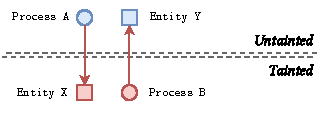
\includegraphics[width=0.55\linewidth]{figures/CitadelTaint.pdf}
    \caption[Accesses across the taint boundary]{Accesses across the taint boundary taint the untainted party.}
    \label{fig:taint-boundary}
\end{figure}

\paragraph{} The \textsc{Citadel} \acrshort{lsm} tracks all entities within the Linux system by attaching a small data structure ($<48$ bytes) to each; it computes and tracks a conservative notion of \textit{taint} for each to ensure \textit{safety}. Tainting in \textsc{Citadel} is dynamic and additive --- entities are only policed if involved in a successful operation crossing the taint boundary (Figure~\ref{fig:taint-boundary}). In additional to automatic propagation, the policy domain may amend the taint for most entities.

\paragraph{} The following metadata is tracked for each entity:

\begin{enumerate}
    \item[---]\textbf{Active}. Processes only --- these require many markers and flags, including; \textit{taint} and its \textit{reservation list}.
    \item[---] \textbf{Passive}. There are many forms of passive entity, the most prevalent being files and other inode-backed structures. These carry \textit{taint}, an \textit{identifier} (tag), and an \textit{anonymous flag}. Non inode-backed tracking is discussed in §~\ref{sec:shm}.
\end{enumerate}

\subsubsection{Identifiers}
\paragraph{} Entities are tagged with a single, randomly-generated 128-bit identifier, A security policy may maintain internal pseudonyms for secrecy and integrity, but must convert back to the system tag for enforcement.

\subsubsection{Extended Attributes} 
\paragraph{} An inode-backed entity's taint flag and identifier are copied to \textit{\acrshort{xattr}s}. These occupy the \texttt{security.citadel} namespace, and ensure that taints and identifiers persist between boots. Certain entities may be \textit{anonymous}, indicated by an anonymous flag, if their identifier is not present as an \textit{\acrshort{xattr}}, either because the entity does not support \textit{\acrshort{xattr}} or those with temporary identifier (§~\ref{sec:entity-creation}).


\subsubsection{Permissions} 
\paragraph{} Tainted processes must hold a valid reservation to perform any operation allowing data to flow to another entity --- enforcement strictly follows the rules in §~\ref{sec:permissible-operations}. Untainted processes bypass all checks, and thus lie outside the \acrshort{ifc} model; security implications are discussed in §~\ref{sec:ifc-model-implications}


\subsubsection{Reservation Cache} 
\paragraph{} When the system's policy enclave presents a new reservation to the \acrshort{lsm}, it is stored in the \textit{reservation cache}. Implemented as a red-black tree, this maps a process's identifier to a linked list of its pending reservations. This intermediary storage is necessary as \acrshort{lsm}s are event-driven, and thus can only access an entity's state when it is presented for review. Before a permission check is carried out, the \acrshort{lsm} updates the process's reservation list by;
\begin{enumerate}
    \item \textit{Installing pending tickets}. All reservations are moved to its internal reservation list, ready for inspection.
    \item \textit{Disposing of expired entries}. When a reservation is inserted into the reservation cache, it is timestamped with an explicit expiry date --- this lifetime is $15$ seconds by default.  
\end{enumerate}


\subsubsection{Entity Creation}
\label{sec:entity-creation}
\paragraph{} Every newly spawned process is privately tagged by the \acrshort{lsm} as if it were a passive entity (§~\ref{sec:transient-entities}). The purpose of this identifier is to enable association any private, passive entities it creates. This includes the file descriptors provided by \texttt{pipe()}, and any new files it creates using \texttt{open()}. Processes always have permission to access their transient entities, and external entities can only gain access rights if they;
\begin{enumerate}
    \item Are a child processes requesting access to their parent, or
    \item The process officially \textit{claims} them via the policy enclave, giving them an independent tag and removing the entity's status as transient. 
\end{enumerate}


\paragraph{\texttt{fork()}} In Linux, child processes are initially exact clones of their parent, with access to the same state and file descriptors. Thus children of tainted processes are also tainted, but importantly without the same rights as their parents --- open file descriptors will not function without revalidation (§~\ref{sec:libcitadel}), and children must request the right to their parent's transient entities to use pipes or similar. It is the policy enclave's responsibility to validate that the security contexts of the parent and child have not diverged. 
% TODO
% \footnote{\textcolor{red}{mention leakage through fd state}}





\subsection{Policy Components}
\label{sec:policy-enclave}

\paragraph{} \texttt{citadeld} represents the policy counterpart to the LSM's enforcement, including the core \acrshort{sgx} enclave. \texttt{citadeld} is modular, hosting an independent policy module sitting on top of an enforcement translation library (Figure~\ref{fig:policy-enclave}).

\subsubsection{Abstract Policy Module}
\paragraph{} The policy module is presented with a simple, event-driven interface; this streamlines their implementation, allowing more emphasis to be put on correctness. Their implementation is based around a single method, through which their permission is sought when required; \texttt{asm\_handle\_request(3)}.


\paragraph{} The simplest possible policy is that any operation is permissible. The request parameter, amongst other things, holds the target identifier and set of operations. 

\vspace{3mm}
\begin{minted}[fontsize=\small]{c}
citadel_response_t asm_handle_request (pid_t pid, 
        struct citadel_op_request *request, void *metadata) {
    return CITADEL_OP_APPROVED;
}
\end{minted}

\begin{figure}[]
    \centering
    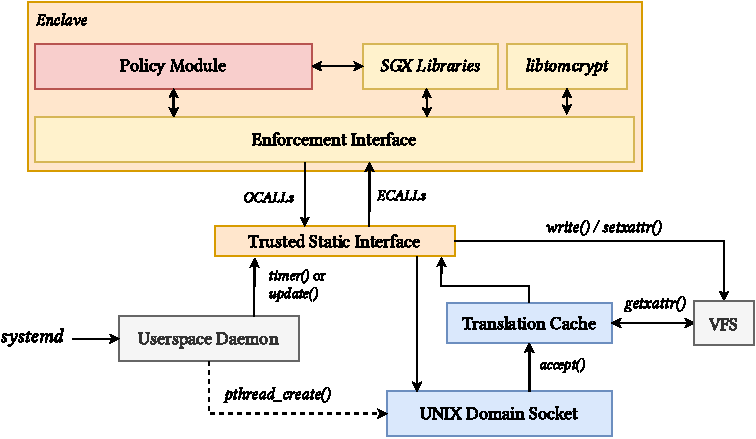
\includegraphics[width=0.9\linewidth]{figures/EnclaveLayout.pdf}
    \caption{Overview of the components inside \texttt{citadeld}.}
    \label{fig:policy-enclave}
\end{figure}

\paragraph{} This can be considered to determine the validity of an operation, $A \xrightharpoonup{\;\omega\;} t$, based on its knowledge of any implicated flows ($A \rightarrow *$).

\paragraph{Operations} Entity operations, $\Omega$, are presented as \texttt{citadel\_operation\_t}, a simple bit mask over the operations \textsc{Citadel} recognises. Similarly, policy decisions are represented using \texttt{citadel\_response\_t}; these may be \textit{approved}, \textit{rejected}, \textit{error}, \textit{invalid}, \textit{granted},\footnote{Approved, and confirming that the process is recognised as the owner of the entity.} and \textit{forged}.\footnote{See §~\ref{sec:additional-security}.}


\subsubsection{Host Application}

\paragraph{} There are several steps before presenting requests to the resident policy module (§~\ref{sec:interdomain-comms}). Requests often refer to absolute filepaths, requiring retrieval of their tags, if they exist --- security \textit{\acrshort{xattr}} serve these requests. Translation is performed pre-emptively depending on the operation requested, and results are cached in a \textit{translation cache} to minimise overhead. This is implemented using \textit{sparsehash},\footnote{\url{https://github.com/sparsehash/sparsehash}} and great care is taken to detect stale entities that may confuse the internal decision process.


\subsubsection{Enforcement Interface}
\paragraph{} The policy module is interchangeable, but the enforcement interface acts as the enclave's backbone. All requests are routed through it to detect forgery or invalid data, and all information leaving it is formatted and signed\footnote{Encryption is discussed in §~\ref{sec:interdomain-comms}} as appropriate. The process of installing reservations created by the enforcement interface is detailed in §~\ref{sec:interdomain-comms}.

\subsubsection{\texttt{libtomcrypt}}
\paragraph{} We ported \textit{libtomcrypt},\footnote{\url{https://github.com/libtom/libtomcrypt}} a leading open-source cryptography library, to function inside an \acrshort{sgx} enclave as \texttt{citadeld} requires many encryption mechanisms on top of those provided by \acrshort{sgx}. Porting was achieved by replacing \textit{libtomcrypt}'s backing precision arithmetic library with an \acrshort{sgx}-aware version of \textit{\acrshort{gmp}},\footnote{\url{https://github.com/intel/sgx-gmp}} and forcing it to statically allocate its memory (as \acrshort{sgx} v1 lacks support for dynamic memory management). Further changes rewrote the internal random number generator to use the one provided by \acrshort{sgx}, and rework its exception strategy to remove \texttt{abort()}, an illegal instruction inside an enclave.

\subsubsection{Shared Memory}
\label{sec:shm}
\paragraph{} \textsc{Citadel} also supports the tagging and restriction of shared memory (\acrshort{shm}). This is managed directly using \textit{System V} identifiers granted to allocated memory segments instead of inodes. Internally, restrictions function as files do, but per-access mediation is not directly possible -- we can only detect when segments are allocated and attached. Thus this workflow requires special consideration, and a new reporting mechanism from the \acrshort{lsm} back to the policy enclave. Using a specialised \textit{\acrshort{xattr}} interface (\ref{eqn:shm-interface}) to drive a request-response model, the \acrshort{lsm} tracks and reports the \acrshort{pid}s of everything that has touched an \acrshort{shm} segment. 

\vspace{-8mm}
\begin{align}
    \texttt{security.citadel.shm.[shm\_id]} \longrightarrow \{145, 267, 1120, ...\} \label{eqn:shm-interface}
\end{align}

\subsection{Communication Pathways}
\label{sec:interdomain-comms}
\paragraph{} There are three notable \acrshort{io} pathways between components within \textsc{Citadel};
\begin{enumerate}
    \item \textsc{Applications $\longleftrightarrow$ Policy Enclave}. \\
    All application requests (via \texttt{libcitadel}, §~\ref{sec:libcitadel}) are sent to the policy enclave using a standard domain socket; \texttt{/run/citadel.socket}. To ensure that all processes can communicate with the reference monitor, a special tag, $\tau = 2^{128} -1$, is assigned, asserting the reference monitor's ownership of it and whitelisting it in the \acrshort{lsm}.
    \vspace{5mm} % TODO hack
    \item \textsc{Policy Enclave $\longleftrightarrow$ \acrshort{lsm}}. \\
    Communication uses two mediums; \textit{SecurityFS} and \textit{\acrshort{xattr}s}. All messages are encrypted using \acrshort{aes}-256-\acrshort{gcm}~\cite{Rijndael,McGrew2005TheGM}; the key is chosen during initialisation (§~\ref{sec:initialisation}). \\
    Reservations are installed using a custom \textit{SecurityFS} interface\footnote{\texttt{/sys/kernel/security/citadel/update}} and synchronously inserted into the reservation cache. The policy enclave may invoke an operation directly on a file using \texttt{setxattr()}, which the LSM intercepts, triggering it to enact the required changes. One common use of this is entity tagging.
    \item \textsc{LSM $\longrightarrow$ Applications}. \\
    To verify their identities with the policy enclave, applications present a \textit{ptoken} with each request (§~\ref{sec:ptokens}) which is generated by reading from a public \textit{SecurityFS} interface.\footnote{\texttt{/sys/kernel/security/citadel/ptoken}} \\
    Additionally, \texttt{libcitadel} occasionally needs to check the tag associated with a path or file descriptor; this is managed using the existing \texttt{libc} \textit{\acrshort{xattr}} methods.
\end{enumerate}

\subsubsection{Initialisation and Encryption}
\label{sec:initialisation}
\paragraph{} Whenever the system boots, the \acrshort{lsm} is first to come online --- \texttt{citadeld} may start any time afterwards, meaning that the \acrshort{lsm} must be capable of operating independently. In this case the system will tend towards a state of complete lockdown (for tainted processes). Thus the mechanism by which the \acrshort{lsm} and policy enclave initialise communication is vital for secure operation; \textsc{Citadel} achieves this with a pair of 2048-bit \acrshort{rsa} keypairs, one for the enclave ($E_{P/S}$) and one for the kernel ($K_{P/S}$).

\paragraph{} \acrshort{sgx} does not provide protection against reverse engineering, thus the enclave's keys must be provided as a sealed entity; sealing here uses \texttt{MRSIGNER}, allowing any policy enclave provided by the \textit{sealing authority} to fully function, and is compiled into the kernel, available via \textit{SecurityFS}.\footnote{\texttt{/sys/kernel/security/citadel/sealed\_keys}}

\paragraph{} Once a policy enclave has been initialised it must verify itself; the \acrshort{lsm} issues a random challenge\footnote{\texttt{/sys/kernel/security/citadel/challenge}} encrypted using the enclave's public key, and expects a reply using the corresponding private key.

\vspace{-5mm}
\begin{align*}
    \text{\acrshort{lsm}} \rightarrow \text{Enclave} &: \{\textit{challenge}\}_{E_{P}} \\
    \text{Enclave} \rightarrow \text{\acrshort{lsm}} &: \{\textit{challenge}, \textit{\acrshort{pid}}, \textit{identifier}, \textit{aes\_key}, ...\}_{K_{P}}
\end{align*}

\paragraph{} Given $E_S$ is only held sealed, any entity providing a valid challenge is trusted and considered part of the \textsc{Citadel} \acrshort{tcb}. The challenger's \acrshort{pid} is stored to detect any adversarial replay messages. \acrshort{rsa} is only used for this initial exchange; it would be too slow to use for all messages. Thus the \acrshort{aes} key provided in the response underlies all future communication.

\paragraph{} \textsc{Citadel} uses \acrshort{aes} for protection as all \acrshort{sgx}-capable processors supports \textit{\acrshort{aesni}};~\cite{aesni} this provides hardware-accelerated \acrshort{aes} operations to achieve an encryption bandwidth over 1 Gbps, far exceeding the capacity required, so adds negligible overhead. The system's \acrshort{aes} key updates with every message sent from the enclave using an \acrshort{sgx}-approved source of entropy;\footnote{$new \leftarrow old \oplus update$} this adds minimal overhead and constitutes good practice. A copy of the first key presented in the challenge-response is retained and used in cases when a static key is essential.

\subsection{\texttt{libcitadel}}
\label{sec:libcitadel}
\paragraph{} \textsc{Citadel} provides a userspace auxiliary library to make integrating existing programs easy and unobtrustive. For each mediated \textit{syscall} (e.g. \texttt{open()}) it provides a proxy function (\texttt{c\_open()}), thus requiring no major changes to applications' workflows.\footnote{Future work would integrate this directly into \texttt{libc}.} A good example of this in action is the ported version of \textit{Nginx} (§~\ref{sec:nginx-benchmarks}). \texttt{libcitadel} performs two main functions;
\begin{enumerate}
    \item Communication with the policy enclave.
    \item Tracking and predicting what permissions it believes the process has.
\end{enumerate}

\paragraph{} Communication is facilitated via \texttt{citadeld}'s domain socket. A zero-copy approach\footnote{Excluding copying in the kernel and transferring the request into the enclave.} helps minimise latency on both sides; this is optimised for in the protocol design. Each communicant verifies the \acrshort{pid} of the other party (§~\ref{sec:ptokens}).

\paragraph{} Caching at this level has a tremendous impact on overall performance. When reading a large file a program may make thousands of calls to \texttt{c\_read()} --- always calling to \texttt{citadeld} would be wasteful, as processes usually have enough information to infer their current position.

\paragraph{} Therefore every process  maintains a list of \textit{expectations} --- the reservations it believes it has, including their validity --- and inferred taint status. They cannot precisely know the true values, especially as the policy enclave may grant different permissions than asked for, but in \textit{Nginx} over 97\% of requests were servable locally in a realistic workload. Using the same workflow, untainted processes speculatively execute operations, again removing the need to involve \texttt{citadeld}. The performance gain of requests served from the cache reduces the overhead from $\mathcal{O}(10\mu s)$ to $\mathcal{O}(100ns)$.


\begin{listing}
\begin{minted}[fontsize=\small]{c}
int c_open(const char *pathname, int oflag, mode_t mode) {
    int fd; bool from_cache = false;
    bool creating = access(pathname, F_OK) < 0 && (oflag & O_CREAT) > 0;
    
    // Pre-emptively attempt access if I suspect I'm not tainted.
    // Alteratively, register a transient file if we're creating it.
    // -- close and reopen to ensure it is independently tagged.
    if (!am_tainted() || creating) {
        fd = open(pathname, oflag, mode);
        if (!am_tainted() && fd > 0)
            return fd;
        if (fd == -1 && errno != -EPERM)
            return -1;
        if (fd != -1)
            close(fd);
    }

    // Request access from the policy enclave. Claim file if not tagged.
    if (!citadel_file_open(pathname, strlen(pathname)+1, &from_cache))
        return -EPERM;

    // Continue as normal.
    fd = open(pathname, oflag, mode);
    citadel_declare_fd(fd, CITADEL_OP_OPEN);
    if (!am_tainted()) set_taint();
    return fd;
}
\end{minted}
\caption{The \texttt{libcitadel} shim function for \texttt{open()}.}
\label{lst:c_open}
\end{listing}

\paragraph{} A core challenge of the cache is relating open file descriptors to the permissions they require. This involves manual work, including fetching its \textit{\acrshort{xattr}} tag with \texttt{fgetxattr()} and estimating the expiration time of the \acrshort{lsm}'s underlying reservation. \texttt{libcitadel} attempts to revalidate tickets before expiry to avoid unexpected drops in service; this is particularly important for applications unaware of \textsc{Citadel}.

\paragraph{} Special care is required with child processes. Children are given a copy of their parent process's state, including its \texttt{libcitadel} cache. Although the \acrshort{lsm} passes no reservations to the child, \texttt{libcitadel} maintains the same \textit{expectation} cache. Entries in it are marked as invalid, to force the child to revalidate a file descriptor before first use. Additionally, we assume that a process trusts the initialisation code of its child, enabling \texttt{libcitadel} to delete the parent's \textit{ptoken} (§~\ref{sec:ptokens}); the \texttt{c\_fork()} function handles this automatically.


\subsection{Additional Security Features}
\label{sec:additional-security}
\paragraph{} \textsc{Citadel} implements additional security mechanisms to reinforce potentially vulnerable aspects of the system. Both the policy enclave and \acrshort{lsm} use a process's \acrshort{pid} as its primary identifier --- \textsc{Citadel} implements two schemes to protect and prove identity.

\subsubsection{\textit{ptokens}}
\label{sec:ptokens}
\paragraph{} Before a process may interact with \texttt{citadeld}, it must retrieve its \textit{ptoken} from the \acrshort{lsm}.\footnote{Read from \texttt{/sys/kernel/security/citadel/ptoken}} The purpose of this (\ref{eqn:ptoken}) is twofold;
\begin{enumerate}
    \item[a.] Inform \texttt{libcitadel} about the process's metadata in the eyes of the \acrshort{lsm}, and
    \item[b.] Provide an authenticable access token to present to \texttt{citadeld}, verifying the process's identity. This encrypted using $K$, the system's designated static \acrshort{aes} key, which is unknown to the process. 
\end{enumerate}

\vspace{-7mm}
\begin{align}
    \textit{ptoken} \rightarrow ( \text{citadel\_pid}, \text{identifier}, \text{token}, \{\text{identifier}, \text{token}, \text{pid}\}_K) \label{eqn:ptoken}
\end{align}

\paragraph{} Whenever a process connects to the \texttt{citadeld} socket, its identity is retrieved from the underlying transport mechanism (Listing~\ref{lst:socket-pid}). At both the sender and receiver the identity of the other is verified using this method, and additionally \texttt{libcitadel} expects the decrypted \textit{token} to be returned by \texttt{citadeld}, inspiring confidence that the response is legitimate.

\begin{listing}
\begin{minted}[fontsize=\small]{c}
// Get PID of sender.
struct ucred cred;
socklen_t len = sizeof(struct ucred);
getsockopt(socket, SOL_SOCKET, SO_PEERCRED, (void*)&cred, &len);
uint64_t pid = cred.pid;
\end{minted}
\vspace{3mm}
\caption[PID retrieval from an active domain socket.]{\acrshort{pid} retrieval from an active domain socket.}
\label{lst:socket-pid}
\end{listing}

\subsubsection{PID Protection}
\label{sec:pid-protection}
\paragraph{} The LSM also watches for \acrshort{pid} forgery, as it is possible for \acrshort{pid}s to be modified with the help of a malicious kernel module (Appendix~\ref{appendix:pid-tampering}). This would be detrimental for the \acrshort{lsm}'s integrity, allowing a process to silently assume another's identity. Therefore the \acrshort{lsm} stores a process's \acrshort{pid} within its security structure and routinely checks to ensure it does not change unexpectedly.\footnote{A valid change would be on \texttt{fork()}, in which case the stored \acrshort{pid} should equal the parent process's.} Any process deemed to have an illegitimate \acrshort{pid} is denied access to all entities, effectively killing it.

\subsection{\textsc{Citadel} Build System}
\label{sec:build-system}
\paragraph{} Building \textsc{Citadel} requires both the kernel and policy enclave to be in agreement about the shared \acrshort{rsa} keys; without this compilation will fail. A preparatory script achieves this by;

\begin{enumerate}
    \item Downloading the kernel's source and inserting the \textsc{Citadel} \acrshort{lsm}.
    \item Generating two \textit{OpenSSL}\footnote{\url{https://www.openssl.org/}} 2048-bit \acrshort{rsa} keys in \textit{\acrshort{der}} format --- the kernel's \textit{Crypto \acrshort{api}} requires keys to present themselves as \textit{\acrshort{asn}.1 structures}.\footnote{\url{https://tls.mbed.org/kb/cryptography/asn1-key-structures-in-der-and-pem}}
    \item Compiling and launching \textsc{Citadel}'s \textit{preparatory enclave}, signed with the same \textit{signing identity} as any policy enclaves generated. This ingests the two keys and generates a sealed keyset to be presented to initialising enclaves.
    \item Generating an interface file (\texttt{keys.h}) in the kernel's source directory --- this file contains the kernel's keypair, the enclave's public key, and the aforementioned sealed keyset. The key files are deleted.
    \item Building and signing the poicy enclaves.
    \item The kernel may now be compiled.
\end{enumerate}
